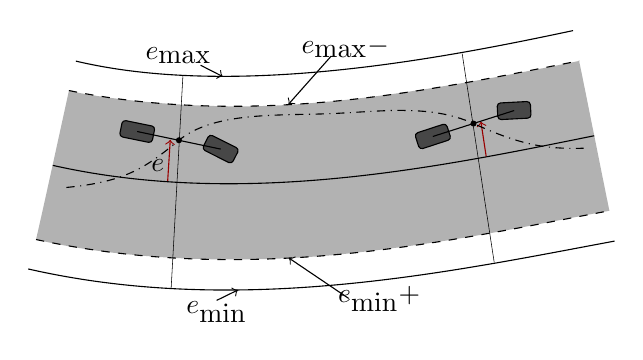
\begin{tikzpicture}[scale = 1.1]
	\tikzset{sref/.style={
			draw = blue,
			%thick, 
			->
			%, >={Latex[length=5pt, width=3pt]}
	},
	elat/.style={
		red!60!black,
		%thick,
		->
		%, >={Latex[length=5pt, width=3pt]}
	},
	elimits/.style={
	->
	%, >={Latex[length=5pt, width=3pt]}
	},
	nplane/.style={
		very thin,
		draw=black
	}
}
%% --------------------- TRACK -----------------------
% FILLED AREA
\draw  [draw opacity=0][fill = black!30] (-1.430,1.400) .. controls (-1.295,1.353) and (0.079,1.126) .. (1.413,1.259) .. controls (2.446,1.339) and (3.866,1.619) .. (4.460,1.742) .. controls (4.513,1.493) and (4.737,0.363) .. (4.810,0.012) .. controls (3.786,-0.174) and (3.079,-0.348) .. (1.613,-0.501) .. controls (0.219,-0.621) and (-1.014,-0.508) .. (-1.810,-0.320) .. controls (-1.736,-0.005) and (-1.466,1.235) .. (-1.430,1.400) -- cycle ;
% CENTERLINE
\draw    (-1.616,0.536) .. controls (0.594,0.038) and (2.894,0.528) .. (4.634,0.878) ;
% E_MAX 
\draw    (-1.350,1.740) .. controls (0.500,1.302) and (2.930,1.782) .. (4.390,2.092) ;
% E_MAX - BO
\draw[dashed]    (-1.430,1.400) .. controls (0.820,0.942) and (2.990,1.462) .. (4.460,1.742) ;
% E_MIN 
\draw    (-1.900,-0.660) .. controls (0.550,-1.218) and (2.990,-0.688) .. (4.870,-0.338) ;
% E_MIN - BO 
\draw[dashed]    (-1.810,-0.320) .. controls (0.700,-0.858) and (2.930,-0.338) .. (4.810,0.012) ;
% NORMAL PLANE 1
\draw  [nplane]  (-0.114,1.573) -- (-0.250,-0.884) ;
% NORMAL PLANE 2 
\draw  [nplane]  (3.110,1.826) -- (3.480,-0.584) ;
% CENTER POINTS' POSITIONS
%\draw    (-0.182,0.344) -- (3.295,0.621) ;

%% --------------------- REF AND DISTANCES -----------------------
% X-AXIS 1
%\draw [sref] (-0.182,0.344) -- (0.097,0.330);
% Y-AXIS 1
%\draw [sref]   (-0.182,0.344) -- (-0.169,0.617) ;
% E-LAT 1
\draw [elat]   (-0.290,0.357) -- (-0.260,0.832) node[midway,black,xshift=-4,yshift=-2] {$e$};;
% X-AXIS 2
%\draw [sref]   (3.295,0.621) -- (3.571,0.661);
% Y-AXIS 2
%\draw [sref]   (3.295,0.621) -- (3.254,0.890) ;
% E-LAT 2
\draw[elat]   (3.387,0.641) -- (3.326,1.042) ;

%% --------------------- VEHICLES -----------------------
% VEHICLE'S COM POSITIONS 
%\draw  (-0.160,0.826) -- (3.241,1.019) ;
\fill (-0.160,0.826) circle (1pt) ;
\fill (3.241,1.019) circle (1pt) ;
% TRAJECTORY
%\draw[dashdotted]    (-1.407,0.809) .. controls (-1.007,1.109) and (-0.560,0.526) .. (-0.160,0.826) .. controls (0.240,1.126) and (0.890,1.084) .. (1.496,1.130) .. controls (2.103,1.177) and (2.666,1.255) .. (3.241,1.019) .. controls (3.816,0.784) and (4.183,0.944) .. (4.296,1.057) ;
\draw[dashdotted]    (-1.460,0.281) .. controls (-0.767,0.347) and (-0.540,0.514) .. (-0.160,0.826) .. controls (0.220,1.137) and (0.886,1.113) .. (1.496,1.130) .. controls (2.107,1.147) and (2.715,1.258) .. (3.241,1.019) .. controls (3.767,0.781) and (4.053,0.721) .. (4.513,0.734) ;
% VEHICLE 1
% CHASSIS 1 
\draw    (-0.642,0.927) -- (0.322,0.724) ;
% FRONT WHEEL 1
\draw  [fill={rgb, 255:red, 0; green, 0; blue, 0 }  ,fill opacity=0.6 ] (0.176,0.862) .. controls (0.186,0.881) and (0.209,0.888) .. (0.228,0.879) -- (0.501,0.742) .. controls (0.521,0.733) and (0.528,0.709) .. (0.519,0.690) -- (0.467,0.587) .. controls (0.457,0.568) and (0.434,0.560) .. (0.415,0.569) -- (0.142,0.706) .. controls (0.122,0.716) and (0.115,0.739) .. (0.124,0.758) -- cycle ;
% REAR WHEEL 1
\draw  [fill={rgb, 255:red, 0; green, 0; blue, 0 }  ,fill opacity=0.6 ] (-0.818,1.022) .. controls (-0.814,1.042) and (-0.793,1.056) .. (-0.772,1.052) -- (-0.473,0.991) .. controls (-0.452,0.987) and (-0.438,0.967) .. (-0.442,0.946) -- (-0.465,0.833) .. controls (-0.469,0.812) and (-0.490,0.798) .. (-0.511,0.802) -- (-0.810,0.863) .. controls (-0.831,0.867) and (-0.845,0.887) .. (-0.841,0.908) -- cycle ;
% VEHICLE 2
% CHASSIS 2 
\draw    (2.772,0.870) -- (3.710,1.169) ;
% FRONT WHEEL 2
\draw  [fill={rgb, 255:red, 0; green, 0; blue, 0 }  ,fill opacity=0.6 ] (3.515,1.217) .. controls (3.514,1.238) and (3.531,1.256) .. (3.552,1.257) -- (3.857,1.273) .. controls (3.879,1.274) and (3.897,1.258) .. (3.898,1.237) -- (3.904,1.121) .. controls (3.905,1.100) and (3.889,1.082) .. (3.868,1.081) -- (3.562,1.065) .. controls (3.541,1.063) and (3.523,1.080) .. (3.521,1.101) -- cycle ;
% REAR WHEEL 2
\draw  [fill={rgb, 255:red, 0; green, 0; blue, 0 }  ,fill opacity=0.6 ] (2.572,0.865) .. controls (2.565,0.886) and (2.576,0.907) .. (2.597,0.914) -- (2.887,1.009) .. controls (2.908,1.016) and (2.929,1.005) .. (2.936,0.985) -- (2.972,0.875) .. controls (2.979,0.854) and (2.968,0.833) .. (2.948,0.826) -- (2.657,0.731) .. controls (2.637,0.724) and (2.615,0.735) .. (2.608,0.755) -- cycle ;

%% --------------------- E-MAX/E-MIN LABELS -----------------------
% E-MAX
\draw[elimits]    (0.090,1.692) -- (0.345,1.562) node[above,xshift = -16,yshift = 1] {$e_\textrm{max}$};
% E-MIN
\draw[elimits]   (0.275,-1.023) node[below,yshift = 3] {$e_\textrm{min}$} -- (0.520,-0.903) ;
% E-MAX - BO
%\draw[elimits]     (0.850,1.372) -- (1.105,1.242) node[above,xshift = -16,yshift = -2] {$e_\textrm{max}-\be$};
\draw[elimits]     (1.6,1.8) node[above,yshift = -4,xshift = 5] {$e_\textrm{max}-\be$} -- (1.105,1.242) ;
% E-MIN - BO
%\draw[elimits]     (0.865,-0.654) -- (1.110,-0.534) ;
\draw[elimits]     (1.8,-1.0) node[below,yshift = 8,xshift = 11] {$e_\textrm{min}+\be$} -- (1.110,-0.534) ;
	
\end{tikzpicture}